\documentclass[10pt,aspectratio=43]{beamer} 
\usepackage{hyperref}
\usepackage{xeCJK} %导入中文包

\setCJKsansfont{SimHei} 
\setsansfont{Times New Roman}
\setmainfont{Microsoft YaHei}
\usefonttheme[onlymath]{serif}
% other packages
\usepackage{latexsym,amsmath,xcolor,multicol,booktabs,calligra}
\usepackage{graphicx,pstricks,listings,stackengine}
\usepackage[linesnumbered,vlined]{algorithm2e}
%\usepackage[linesnumbered,ruled,vlined]{algorithm2e}
\usepackage{float}    
\author{雷尚远}
\title{定向覆盖模糊测试工具的设计与实现}
\subtitle{毕业设计中期检查}
\institute{南京邮电大学计算机学院}
\date{2023年4月17日}
\usepackage{NJUPT}

% defs
\def\cmd#1{\texttt{\color{red}\footnotesize $\backslash$#1}}
\def\env#1{\texttt{\color{blue}\footnotesize #1}}
\definecolor{deepblue}{rgb}{0,0,0.5}
\definecolor{deepred}{rgb}{0.6,0,0}
\definecolor{deepgreen}{rgb}{0,0.5,0}
\definecolor{halfgray}{gray}{0.55}

\lstset{
    basicstyle=\ttfamily\small,
    keywordstyle=\bfseries\color{deepblue},
    emphstyle=\ttfamily\color{deepred},    % Custom highlighting style
    stringstyle=\color{deepgreen},
    numbers=left,
    numberstyle=\small\color{halfgray},
    rulesepcolor=\color{red!20!green!20!blue!20},
    frame=shadowbox,
}


\begin{document}

\begin{frame}
    \titlepage
    \begin{figure}[htpb]
        \begin{center}
            
\includegraphics[width=0.2\linewidth]{pic/NJUPT_Logo.pdf}
        \end{center}
    \end{figure}
\end{frame}

\begin{frame}
    \tableofcontents[sectionstyle=show,subsectionstyle=show/shaded/hide,subsubsectionstyle=show/shaded/hide]
\end{frame}


\section{Background}
\subsection{Pre-Knowledge}
\begin{frame}[fragile] {What Fuzzing is?}
    \only<1>{
        \structure {Defination\cite{manes2019art}}
        \begin{itemize} 
            \item \textbf{Fuzzing} Fuzzing is the execution of the PUT using input(s) sampled from an input space (the “fuzz input space”) 
                that protrudes the expected input space of the PUT.
                \\ - PUT: Program Under Test
            \item \textbf{Fuzz testing} Fuzz testing is the use of fuzzing to test if a PUT violates a correctness policy.
            \item \textbf{Fuzzer} A fuzzer is a program that performs fuzz testing on a PUT.
            \item \textbf{Bug Oracle} A bug oracle is a program, perhaps as part of a fuzzer, that determines whether a given execution 
            of the PUT violates a specific correctness policy.
            \item \textbf{Fuzz Configuration}  A fuzz configuration of a fuzz algorithm comprises the parameter value(s) that control(s) the fuzz algorithm.
            \item \textbf{Seed} A seed is a (commonly well-structured) input to the PUT, used to generate test cases by modifying it.
        \end{itemize}
    } 
    \only<2>{
            \begin{block}{Fuzz Testing}
            \begin{algorithm}[H]
                \small
                \DontPrintSemicolon
                \SetKwSty{algokeywordsty}
                \SetFuncSty{algofuncsty}
                \SetDataSty{algodatasty}
                \SetArgSty{algoargsty}
                \SetCommentSty{algocmtsty}
                \SetKw{break}{break}
                \SetKw{not}{not}
                \SetKwFunction{preprocess}{\textsc{Preprocess}}
                \SetKwFunction{schedule}{\textsc{Schedule}}
                \SetKwFunction{inputGen}{\textsc{InputGen}}
                \SetKwFunction{inputEval}{\textsc{InputEval}}
                \SetKwFunction{confUpdate}{\textsc{ConfUpdate}}
                \SetKwFunction{continue}{\textsc{Continue}}
                \SetKwFunction{isBug}{isBug}
                \SetKwFunction{getProgram}{getProgram}
                \SetKwData{newbugs}{$\bugs^\prime$}
                \KwIn{\confs, \timeout}
                \KwOut{\bugs \tcp{a finite set of bugs}}
                $\bugs \gets \varnothing$\;
                $\confs \gets \preprocess{$\confs$}$\;
                \While {$\currtime < \timeout \land \continue{\confs}$}{
                  \conf $\gets \schedule{\confs, \currtime, \timeout}$\;
                  \testcases $\gets \inputGen{\conf}$\;
                  \tcp{\bugoracle is embedded in a fuzzer}
                  \newbugs, \execinfos $\gets$ \inputEval{\conf, \testcases, \bugoracle}\;
                  $\confs \gets \confUpdate{\confs, \conf, \execinfos}$\;
                  $\bugs \gets \bugs \cup \newbugs$\;
                }
                \Return{\bugs}\;
                %\caption[short]{fuzz testing}
            \end{algorithm} 
        \end{block}
    } 
\end{frame}

\begin{frame}{Fuzzing Algorithm}
    \only<1>{
        \begin{minipage}[t]{0.57\textwidth}
        \vspace{0pt}
        \centering
        \begin{algorithm}[H]
            \scriptsize
            \DontPrintSemicolon
            \SetKwSty{algokeywordsty}
            \SetFuncSty{algofuncsty}
            \SetDataSty{algodatasty}
            \SetArgSty{algoargsty}
            \SetCommentSty{algocmtsty}
            \SetKw{break}{break}
            \SetKw{not}{not}
            \SetKwFunction{preprocess}{\textsc{Preprocess}}
            \SetKwFunction{schedule}{\textsc{Schedule}}
            \SetKwFunction{inputGen}{\textsc{InputGen}}
            \SetKwFunction{inputEval}{\textsc{InputEval}}
            \SetKwFunction{confUpdate}{\textsc{ConfUpdate}}
            \SetKwFunction{continue}{\textsc{Continue}}
            \SetKwFunction{isBug}{isBug}
            \SetKwFunction{getProgram}{getProgram}
            \SetKwData{newbugs}{$\bugs^\prime$}
            \HiLi \KwIn{\confs, \timeout}
            \HiLi \KwOut{\bugs \tcp{a finite set of bugs}}
            $\bugs \gets \varnothing$\;
            $\confs \gets \preprocess{$\confs$}$\;
            \While {$\currtime < \timeout \land \continue{\confs}$}{
              \conf $\gets \schedule{\confs, \currtime, \timeout}$\;
              \testcases $\gets \inputGen{\conf}$\;
              \tcp{\bugoracle is embedded in a fuzzer}
              \newbugs, \execinfos $\gets$ \inputEval{\conf, \testcases, \bugoracle}\;
              $\confs \gets \confUpdate{\confs, \conf, \execinfos}$\;
              $\bugs \gets \bugs \cup \newbugs$\;
            }
            \Return{\bugs}\;
        \end{algorithm} 
        \end{minipage} 
        \begin{minipage}[t]{0.4\textwidth}
            {
                \vspace{25pt}
                \centering
                \footnotesize{
                    \begin{itemize}  
                        \item  \confs :a set of fuzz configurations
                        \item  \timeout: timeout
                        \item  \bugs: a set of discovered bugs
                    \end{itemize} 
                }
            }
        \end{minipage}
    }  

    \only<2>{
        \begin{minipage}[t]{0.57\linewidth}
        \vspace{0pt}
        \centering
        \begin{algorithm}[H]
            \scriptsize
            \DontPrintSemicolon
            \SetKwSty{algokeywordsty}
            \SetFuncSty{algofuncsty}
            \SetDataSty{algodatasty}
            \SetArgSty{algoargsty}
            \SetCommentSty{algocmtsty}
            \SetKw{break}{break}
            \SetKw{not}{not}
            \SetKwFunction{preprocess}{\textsc{Preprocess}}
            \SetKwFunction{schedule}{\textsc{Schedule}}
            \SetKwFunction{inputGen}{\textsc{InputGen}}
            \SetKwFunction{inputEval}{\textsc{InputEval}}
            \SetKwFunction{confUpdate}{\textsc{ConfUpdate}}
            \SetKwFunction{continue}{\textsc{Continue}}
            \SetKwFunction{isBug}{isBug}
            \SetKwFunction{getProgram}{getProgram}
            \SetKwData{newbugs}{$\bugs^\prime$}
            \KwIn{\confs, \timeout}
            \KwOut{\bugs \tcp{a finite set of bugs}}
            \HiLi$\bugs \gets \varnothing$\;
            \HiLi$\confs \gets \preprocess{$\confs$}$\;
            \While {$\currtime < \timeout \land \continue{\confs}$}{
              \conf $\gets \schedule{\confs, \currtime, \timeout}$\;
              \testcases $\gets \inputGen{\conf}$\;
              \tcp{\bugoracle is embedded in a fuzzer}
              \newbugs, \execinfos $\gets$ \inputEval{\conf, \testcases, \bugoracle}\;
              $\confs \gets \confUpdate{\confs, \conf, \execinfos}$\;
              $\bugs \gets \bugs \cup \newbugs$\;
            }
            \Return{\bugs}\;
        \end{algorithm} 
        \end{minipage} 
        \begin{minipage}[t]{0.4\linewidth}
            \vspace{0pt}
            \centering
            \preprocess\normalfont(\confs) $\rightarrow \confs$ 
            \scriptsize{
            \begin{itemize}
                \item  \textbf{Instrumentation}
                    \\- grey-box and white-box fuzzers
                    \\- \alert{static}/dynamic(\inputEval)
                \item \textbf{Seed Selection}
                    \\- weed out potentially redundant configurations
                \item  \textbf{Seed Trimming}
                    \\- reduce the size of seeds
                \item  \textbf{Preparing a Driver Application}
                     \\- library Fuzzing, kernal Fuzzing
            \end{itemize}
            } 
        \end{minipage}
    }
   
    \only<3>{
        \begin{minipage}[t]{0.57\linewidth}
        \vspace{0pt}
        \centering
        \begin{algorithm}[H]
            \scriptsize
            \DontPrintSemicolon
            \SetKwSty{algokeywordsty}
            \SetFuncSty{algofuncsty}
            \SetDataSty{algodatasty}
            \SetArgSty{algoargsty}
            \SetCommentSty{algocmtsty}
            \SetKw{break}{break}
            \SetKw{not}{not}
            \SetKwFunction{preprocess}{\textsc{Preprocess}}
            \SetKwFunction{schedule}{\textsc{Schedule}}
            \SetKwFunction{inputGen}{\textsc{InputGen}}
            \SetKwFunction{inputEval}{\textsc{InputEval}}
            \SetKwFunction{confUpdate}{\textsc{ConfUpdate}}
            \SetKwFunction{continue}{\textsc{Continue}}
            \SetKwFunction{isBug}{isBug}
            \SetKwFunction{getProgram}{getProgram}
            \SetKwData{newbugs}{$\bugs^\prime$}
            \KwIn{\confs, \timeout}
            \KwOut{\bugs \tcp{a finite set of bugs}}
            $\bugs \gets \varnothing$\;
            $\confs \gets \preprocess{$\confs$}$\;
            \HiLi\While {$\currtime < \timeout \land \continue{\confs}$}{
              \conf $\gets \schedule{\confs, \currtime, \timeout}$\;
              \testcases $\gets \inputGen{\conf}$\;
              \tcp{\bugoracle is embedded in a fuzzer}
              \newbugs, \execinfos $\gets$ \inputEval{\conf, \testcases, \bugoracle}\;
              $\confs \gets \confUpdate{\confs, \conf, \execinfos}$\;
              $\bugs \gets \bugs \cup \newbugs$\;
            }
            \Return{\bugs}\;
        \end{algorithm} 
        \end{minipage}
        \begin{minipage}[t]{0.4\linewidth}
            {
                \vspace{25pt}
                \centering
                    Stop Condition
                    \scriptsize{
                        \begin{itemize}  
                            \item  $\currtime < \timeout$
                            \item  \continue\normalfont(\confs)$\rightarrow \{\texttt{True}, \texttt{False}\}$
                            \\- Determine whether a new fuzz iteration should occur
                        \end{itemize} 
                    }
            }
        \end{minipage}
    }

    \only<4>{
        \begin{minipage}[t]{0.57\linewidth}
        \vspace{0pt}
        \centering
        \begin{algorithm}[H]
            \scriptsize
            \DontPrintSemicolon
            \SetKwSty{algokeywordsty}
            \SetFuncSty{algofuncsty}
            \SetDataSty{algodatasty}
            \SetArgSty{algoargsty}
            \SetCommentSty{algocmtsty}
            \SetKw{break}{break}
            \SetKw{not}{not}
            \SetKwFunction{preprocess}{\textsc{Preprocess}}
            \SetKwFunction{schedule}{\textsc{Schedule}}
            \SetKwFunction{inputGen}{\textsc{InputGen}}
            \SetKwFunction{inputEval}{\textsc{InputEval}}
            \SetKwFunction{confUpdate}{\textsc{ConfUpdate}}
            \SetKwFunction{continue}{\textsc{Continue}}
            \SetKwFunction{isBug}{isBug}
            \SetKwFunction{getProgram}{getProgram}
            \SetKwData{newbugs}{$\bugs^\prime$}
            \KwIn{\confs, \timeout}
            \KwOut{\bugs \tcp{a finite set of bugs}}
            $\bugs \gets \varnothing$\;
            $\confs \gets \preprocess{$\confs$}$\;
            \While {$\currtime < \timeout \land \continue{\confs}$}{
             \HiLi  \conf $\gets \schedule{\confs, \currtime, \timeout}$\;
              \testcases $\gets \inputGen{\conf}$\;
              \tcp{\bugoracle is embedded in a fuzzer}
              \newbugs, \execinfos $\gets$ \inputEval{\conf, \testcases, \bugoracle}\;
              $\confs \gets \confUpdate{\confs, \conf, \execinfos}$\;
              $\bugs \gets \bugs \cup \newbugs$\;
            }
            \Return{\bugs}\;
        \end{algorithm} 
        \end{minipage} 
        \begin{minipage}[t]{0.4\linewidth}
            {
                \vspace{0pt}
                \centering
                \scriptsize{
                \schedule\normalfont(\confs, \currtime, \timeout) $\rightarrow \conf$
                    \begin{itemize} 
                        \item \textbf{Function}
                            \\- Pick important information(\conf )
                        \item \textbf{FCS Problem} 
                            \\- \textit{exploration}:Spent time on gathering more accurate information on each configuration to inform future decisions
                            \\- \textit{exploitation}:Spent time on fuzzing the configurations that are currently believed to lead to more favorable outcomes
                    \end{itemize} 
                }
            }
        \end{minipage}
    }


    \only<5>{
        \begin{minipage}[t]{0.57\linewidth}
        \vspace{0pt}
        \centering
        \begin{algorithm}[H]
            \scriptsize
            \DontPrintSemicolon
            \SetKwSty{algokeywordsty}
            \SetFuncSty{algofuncsty}
            \SetDataSty{algodatasty}
            \SetArgSty{algoargsty}
            \SetCommentSty{algocmtsty}
            \SetKw{break}{break}
            \SetKw{not}{not}
            \SetKwFunction{preprocess}{\textsc{Preprocess}}
            \SetKwFunction{schedule}{\textsc{Schedule}}
            \SetKwFunction{inputGen}{\textsc{InputGen}}
            \SetKwFunction{inputEval}{\textsc{InputEval}}
            \SetKwFunction{confUpdate}{\textsc{ConfUpdate}}
            \SetKwFunction{continue}{\textsc{Continue}}
            \SetKwFunction{isBug}{isBug}
            \SetKwFunction{getProgram}{getProgram}
            \SetKwData{newbugs}{$\bugs^\prime$}
            \KwIn{\confs, \timeout}
            \KwOut{\bugs \tcp{a finite set of bugs}}
            $\bugs \gets \varnothing$\;
            $\confs \gets \preprocess{$\confs$}$\;
            \While {$\currtime < \timeout \land \continue{\confs}$}{
            \conf $\gets \schedule{\confs, \currtime, \timeout}$\;
            \HiLi\testcases $\gets \inputGen{\conf}$\;
              \tcp{\bugoracle is embedded in a fuzzer}
              \newbugs, \execinfos $\gets$ \inputEval{\conf, \testcases, \bugoracle}\;
              $\confs \gets \confUpdate{\confs, \conf, \execinfos}$\;
              $\bugs \gets \bugs \cup \newbugs$\;
            }
            \Return{\bugs}\;
        \end{algorithm} 
        \end{minipage} 
        \begin{minipage}[t]{0.4\linewidth}
            {
                \vspace{25pt}
                \centering
                \scriptsize{
                    \inputGen\normalfont(\conf)$\rightarrow \testcases$ 
                    \begin{itemize}  
                        \item \textbf{function}
                            \\- Generate testcases
                        \item  \textbf{classification}
                            \\- Generation-based(\textit{Model-based})
                            \\- Mutation-based(\textit{Model-less})
                    \end{itemize} 
                }
            }
        \end{minipage}
    }

    \only<6>{
        \begin{minipage}[t]{0.57\linewidth}
        \vspace{0pt}
        \centering
        \begin{algorithm}[H]
            \scriptsize
            \DontPrintSemicolon
            \SetKwSty{algokeywordsty}
            \SetFuncSty{algofuncsty}
            \SetDataSty{algodatasty}
            \SetArgSty{algoargsty}
            \SetCommentSty{algocmtsty}
            \SetKw{break}{break}
            \SetKw{not}{not}
            \SetKwFunction{preprocess}{\textsc{Preprocess}}
            \SetKwFunction{schedule}{\textsc{Schedule}}
            \SetKwFunction{inputGen}{\textsc{InputGen}}
            \SetKwFunction{inputEval}{\textsc{InputEval}}
            \SetKwFunction{confUpdate}{\textsc{ConfUpdate}}
            \SetKwFunction{continue}{\textsc{Continue}}
            \SetKwFunction{isBug}{isBug}
            \SetKwFunction{getProgram}{getProgram}
            \SetKwData{newbugs}{$\bugs^\prime$}
            \KwIn{\confs, \timeout}
            \KwOut{\bugs \tcp{a finite set of bugs}}
            $\bugs \gets \varnothing$\;
            $\confs \gets \preprocess{$\confs$}$\;
            \While {$\currtime < \timeout \land \continue{\confs}$}{
            \conf $\gets \schedule{\confs, \currtime, \timeout}$\;
              \testcases $\gets \inputGen{\conf}$\;
              \tcp{\bugoracle is embedded in a fuzzer}
              \HiLi  \newbugs, \execinfos $\gets$ \inputEval{\conf, \testcases, \bugoracle}\;
              $\confs \gets \confUpdate{\confs, \conf, \execinfos}$\;
              $\bugs \gets \bugs \cup \newbugs$\;
            }
            \Return{\bugs}\;
        \end{algorithm} 
        \end{minipage} 
        \begin{minipage}[t]{0.4\linewidth}
            {
                \vspace{0pt}
                \centering
                \scriptsize{
                    \inputEval\normalfont(\conf, \testcases, \bugoracle) $\rightarrow \bugs^\prime, \execinfos$  
                    \begin{itemize}  
                        \item \textbf{Fuzzing PUT}
                            \\- \testcases
                            \\- $\bugs^\prime$
                        \item \textbf{Feedback Information} 
                            \\- \conf, \testcases
                            \\- \execinfos (\testcases,crashes,stack backtrace hash,edge coverage,etc.)
                    \end{itemize} 
                }
            }
        \end{minipage}
    }

    \only<7>{
        \begin{minipage}[t]{0.57\linewidth}
        \vspace{0pt}
        \centering
        \begin{algorithm}[H]
            \scriptsize
            \DontPrintSemicolon
            \SetKwSty{algokeywordsty}
            \SetFuncSty{algofuncsty}
            \SetDataSty{algodatasty}
            \SetArgSty{algoargsty}
            \SetCommentSty{algocmtsty}
            \SetKw{break}{break}
            \SetKw{not}{not}
            \SetKwFunction{preprocess}{\textsc{Preprocess}}
            \SetKwFunction{schedule}{\textsc{Schedule}}
            \SetKwFunction{inputGen}{\textsc{InputGen}}
            \SetKwFunction{inputEval}{\textsc{InputEval}}
            \SetKwFunction{confUpdate}{\textsc{ConfUpdate}}
            \SetKwFunction{continue}{\textsc{Continue}}
            \SetKwFunction{isBug}{isBug}
            \SetKwFunction{getProgram}{getProgram}
            \SetKwData{newbugs}{$\bugs^\prime$}
            \KwIn{\confs, \timeout}
            \KwOut{\bugs \tcp{a finite set of bugs}}
            $\bugs \gets \varnothing$\;
            $\confs \gets \preprocess{$\confs$}$\;
            \While {$\currtime < \timeout \land \continue{\confs}$}{
            \conf $\gets \schedule{\confs, \currtime, \timeout}$\;
              \testcases $\gets \inputGen{\conf}$\;
              \tcp{\bugoracle is embedded in a fuzzer}
              \newbugs, \execinfos $\gets$ \inputEval{\conf, \testcases, \bugoracle}\;
              \HiLi  $\confs \gets \confUpdate{\confs, \conf, \execinfos}$\;
              \HiLi $\bugs \gets \bugs \cup \newbugs$\;
            }
            \Return{\bugs}\;
        \end{algorithm} 
        \end{minipage} 
        \begin{minipage}[t]{0.4\linewidth}
            {
                \vspace{25pt}
                \centering
                \scriptsize{
                    \begin{itemize}  
                        \item  \confUpdate\normalfont(\confs, \conf, \execinfos) $\rightarrow \confs$
                            \\- Update Fuzz Configuration(distinguishablity)
                            \\- Seed Pool Update
                        \item   $\bugs \cup \bugs^\prime \rightarrow \bugs$
                            \\- Update Bugs Set
                    \end{itemize} 
                }
            }
        \end{minipage}
    }

    \only<8>{
        \begin{minipage}[t]{0.57\linewidth}
        \vspace{0pt}
        \centering
        \begin{algorithm}[H]
            \scriptsize
            \DontPrintSemicolon
            \SetKwSty{algokeywordsty}
            \SetFuncSty{algofuncsty}
            \SetDataSty{algodatasty}
            \SetArgSty{algoargsty}
            \SetCommentSty{algocmtsty}
            \SetKw{break}{break}
            \SetKw{not}{not}
            \SetKwFunction{preprocess}{\textsc{Preprocess}}
            \SetKwFunction{schedule}{\textsc{Schedule}}
            \SetKwFunction{inputGen}{\textsc{InputGen}}
            \SetKwFunction{inputEval}{\textsc{InputEval}}
            \SetKwFunction{confUpdate}{\textsc{ConfUpdate}}
            \SetKwFunction{continue}{\textsc{Continue}}
            \SetKwFunction{isBug}{isBug}
            \SetKwFunction{getProgram}{getProgram}
            \SetKwData{newbugs}{$\bugs^\prime$}
            \KwIn{\confs, \timeout}
            \KwOut{\bugs \tcp{a finite set of bugs}}
            $\bugs \gets \varnothing$\;
            $\confs \gets \preprocess{$\confs$}$\;
            \HiLi\While {$\currtime < \timeout \land \continue{\confs}$}{
              \conf $\gets \schedule{\confs, \currtime, \timeout}$\;
              \testcases $\gets \inputGen{\conf}$\;
              \tcp{\bugoracle is embedded in a fuzzer}
              \newbugs, \execinfos $\gets$ \inputEval{\conf, \testcases, \bugoracle}\;
              $\confs \gets \confUpdate{\confs, \conf, \execinfos}$\;
              $\bugs \gets \bugs \cup \newbugs$\;
            }
            \HiLi\Return{\bugs}\;
        \end{algorithm} 
        \end{minipage} 
        \begin{minipage}[t]{0.4\linewidth}
            {
                \vspace{25pt}
                \centering
                stop condition
                \scriptsize{
                    \begin{itemize}  
                        \item  $\currtime < \timeout$
                        \item  \continue\normalfont(\confs)$\rightarrow \{\texttt{True}, \texttt{False}\}$
                        \\- Determine whether a new fuzz iteration should occur
                    \end{itemize} 
                }
            }
        \end{minipage}
    }
\end{frame}

\subsection{Motivation}
\begin{frame}{Classification}
    \only<1>{
        \begin{quote}
           The amount of collected information defines the color of a fuzzer\cite{manes2019art}.
        \end{quote}
        \begin{minipage}[t]{0.57\linewidth}
        \vspace{0pt}
        \centering
        \begin{algorithm}[H]
            \scriptsize
            \DontPrintSemicolon
            \SetKwSty{algokeywordsty}
            \SetFuncSty{algofuncsty}
            \SetDataSty{algodatasty}
            \SetArgSty{algoargsty}
            \SetCommentSty{algocmtsty}
            \SetKw{break}{break}
            \SetKw{not}{not}
            \SetKwFunction{preprocess}{\textsc{Preprocess}}
            \SetKwFunction{schedule}{\textsc{Schedule}}
            \SetKwFunction{inputGen}{\textsc{InputGen}}
            \SetKwFunction{inputEval}{\textsc{InputEval}}
            \SetKwFunction{confUpdate}{\textsc{ConfUpdate}}
            \SetKwFunction{continue}{\textsc{Continue}}
            \SetKwFunction{isBug}{isBug}
            \SetKwFunction{getProgram}{getProgram}
            \SetKwData{newbugs}{$\bugs^\prime$}
            \KwIn{\confs, \timeout}
            \KwOut{\bugs \tcp{a finite set of bugs}}
            $\bugs \gets \varnothing$\;
            \HiLi$\confs \gets \preprocess{$\confs$}$\;
            \While {$\currtime < \timeout \land \continue{\confs}$}{
              \conf $\gets \schedule{\confs, \currtime, \timeout}$\;
              \testcases $\gets \inputGen{\conf}$\;
              \tcp{\bugoracle is embedded in a fuzzer}
              \newbugs, \execinfos $\gets$ \inputEval{\conf, \testcases, \bugoracle}\;
            \HiLi $\confs \gets \confUpdate{\confs, \conf, \execinfos}$\;
              $\bugs \gets \bugs \cup \newbugs$\;
            }
            \Return{\bugs}\;
        \end{algorithm} 
        \end{minipage} 
        \begin{minipage}[t]{0.4\linewidth}
            \vspace{0pt}
            \centering 
            \scriptsize{
            \begin{itemize}
                \item  \textbf{program instrumentation}
                \scriptsize{
                    \begin{itemize}
                         \item static
                         \item dynamic 
                    \end{itemize}
                }
                \item processor traces
                \item system call usage
                \item etc.
            \end{itemize}
            } 
        \end{minipage}
    }
    \only<2>{
        \begin{minipage}[t]{0.57\linewidth}
        \vspace{0pt}
        \centering
        \begin{algorithm}[H]
            \scriptsize
            \DontPrintSemicolon
            \SetKwSty{algokeywordsty}
            \SetFuncSty{algofuncsty}
            \SetDataSty{algodatasty}
            \SetArgSty{algoargsty}
            \SetCommentSty{algocmtsty}
            \SetKw{break}{break}
            \SetKw{not}{not}
            \SetKwFunction{preprocess}{\textsc{Preprocess}}
            \SetKwFunction{schedule}{\textsc{Schedule}}
            \SetKwFunction{inputGen}{\textsc{InputGen}}
            \SetKwFunction{inputEval}{\textsc{InputEval}}
            \SetKwFunction{confUpdate}{\textsc{ConfUpdate}}
            \SetKwFunction{continue}{\textsc{Continue}}
            \SetKwFunction{isBug}{isBug}
            \SetKwFunction{getProgram}{getProgram}
            \SetKwData{newbugs}{$\bugs^\prime$}
            \KwIn{\confs, \timeout}
            \KwOut{\bugs \tcp{a finite set of bugs}}
            $\bugs \gets \varnothing$\;
            \alert{$\confs \gets \preprocess{$\confs$}$\;}
            \While {$\currtime < \timeout \land \continue{\confs}$}{
              \conf $\gets \schedule{\confs, \currtime, \timeout}$\;
              \testcases $\gets \inputGen{\conf}$\;
              \tcp{\bugoracle is embedded in a fuzzer}
              \newbugs, \execinfos $\gets$ \inputEval{\conf, \testcases, \bugoracle}\;
              $\confs \gets \confUpdate{\confs, \conf, \execinfos}$\;
              $\bugs \gets \bugs \cup \newbugs$\;
            }
            \Return{\bugs}\;
        \end{algorithm} 
        \end{minipage} 
        \begin{minipage}[t]{0.4\linewidth}
            \vspace{0pt}
            \centering 
            \textbf{Program Instrumentation}
            \scriptsize{
                \begin{itemize}
                    \item \alert{Static}
                        \\- source code
                        \\- intermediate code
                        \\- binary-level 
                    \item Dynamic 
                \end{itemize}
                }
        \end{minipage}
    }
    \only<3>{
        \begin{minipage}[t]{0.57\linewidth}
        \vspace{0pt}
        \centering
        \begin{algorithm}[H]
            \scriptsize
            \DontPrintSemicolon
            \SetKwSty{algokeywordsty}
            \SetFuncSty{algofuncsty}
            \SetDataSty{algodatasty}
            \SetArgSty{algoargsty}
            \SetCommentSty{algocmtsty}
            \SetKw{break}{break}
            \SetKw{not}{not}
            \SetKwFunction{preprocess}{\textsc{Preprocess}}
            \SetKwFunction{schedule}{\textsc{Schedule}}
            \SetKwFunction{inputGen}{\textsc{InputGen}}
            \SetKwFunction{inputEval}{\textsc{InputEval}}
            \SetKwFunction{confUpdate}{\textsc{ConfUpdate}}
            \SetKwFunction{continue}{\textsc{Continue}}
            \SetKwFunction{isBug}{isBug}
            \SetKwFunction{getProgram}{getProgram}
            \SetKwData{newbugs}{$\bugs^\prime$}
            \KwIn{\confs, \timeout}
            \KwOut{\bugs \tcp{a finite set of bugs}}
            $\bugs \gets \varnothing$\;
            $\confs \gets \preprocess{$\confs$}$\;
            \While {$\currtime < \timeout \land \continue{\confs}$}{
              \conf $\gets \schedule{\confs, \currtime, \timeout}$\;
              \testcases $\gets \inputGen{\conf}$\;
              \tcp{\bugoracle is embedded in a fuzzer}
            \alert{\newbugs, \execinfos $\gets$ \inputEval{\conf, \testcases, \bugoracle}\;}
              $\confs \gets \confUpdate{\confs, \conf, \execinfos}$\;
              $\bugs \gets \bugs \cup \newbugs$\;
            }
            \Return{\bugs}\;
        \end{algorithm} 
        \end{minipage} 
        \begin{minipage}[t]{0.4\linewidth}
            \vspace{0pt}
            \centering 
            \textbf{Program Instrumentation}
            \scriptsize{
                \begin{itemize}
                    \item Static
                    \item \alert{Dynamic} 
                        \\- 
                        \\-
                \end{itemize}
                }
        \end{minipage}
    }
    \only<4>{
        \structure {Classification of Fuzzing}
        \begin{itemize} 
            \item  \textbf{Black-box Fuzzing}
                \\ - no program analysis, no feedback
            \item  \textbf{White-box Fuzzing} 
                \\ - mostly program analysis
            \item  \textbf{Grey-box  Fuzzing} 
                \\ - no program analysis, but feedback
        \end{itemize} 
    }
\end{frame}
\begin{frame}{Why Grey-box Fuzzing ?}
    \only<1>{
        \begin{itemize}  
        \item \structure {Black-box Fuzzing}
        \\ \textbf{Defination:} techniques that do not see the internals of the PUT,and can observe only the input/output behavior of the PUT,
           treating it as a black-box\cite{manes2019art}.
        \\ -No \alert{program analysis}, no \alert{feedback}
        \end{itemize} 
        \begin{picture}(320,250)
            \put(-15,110){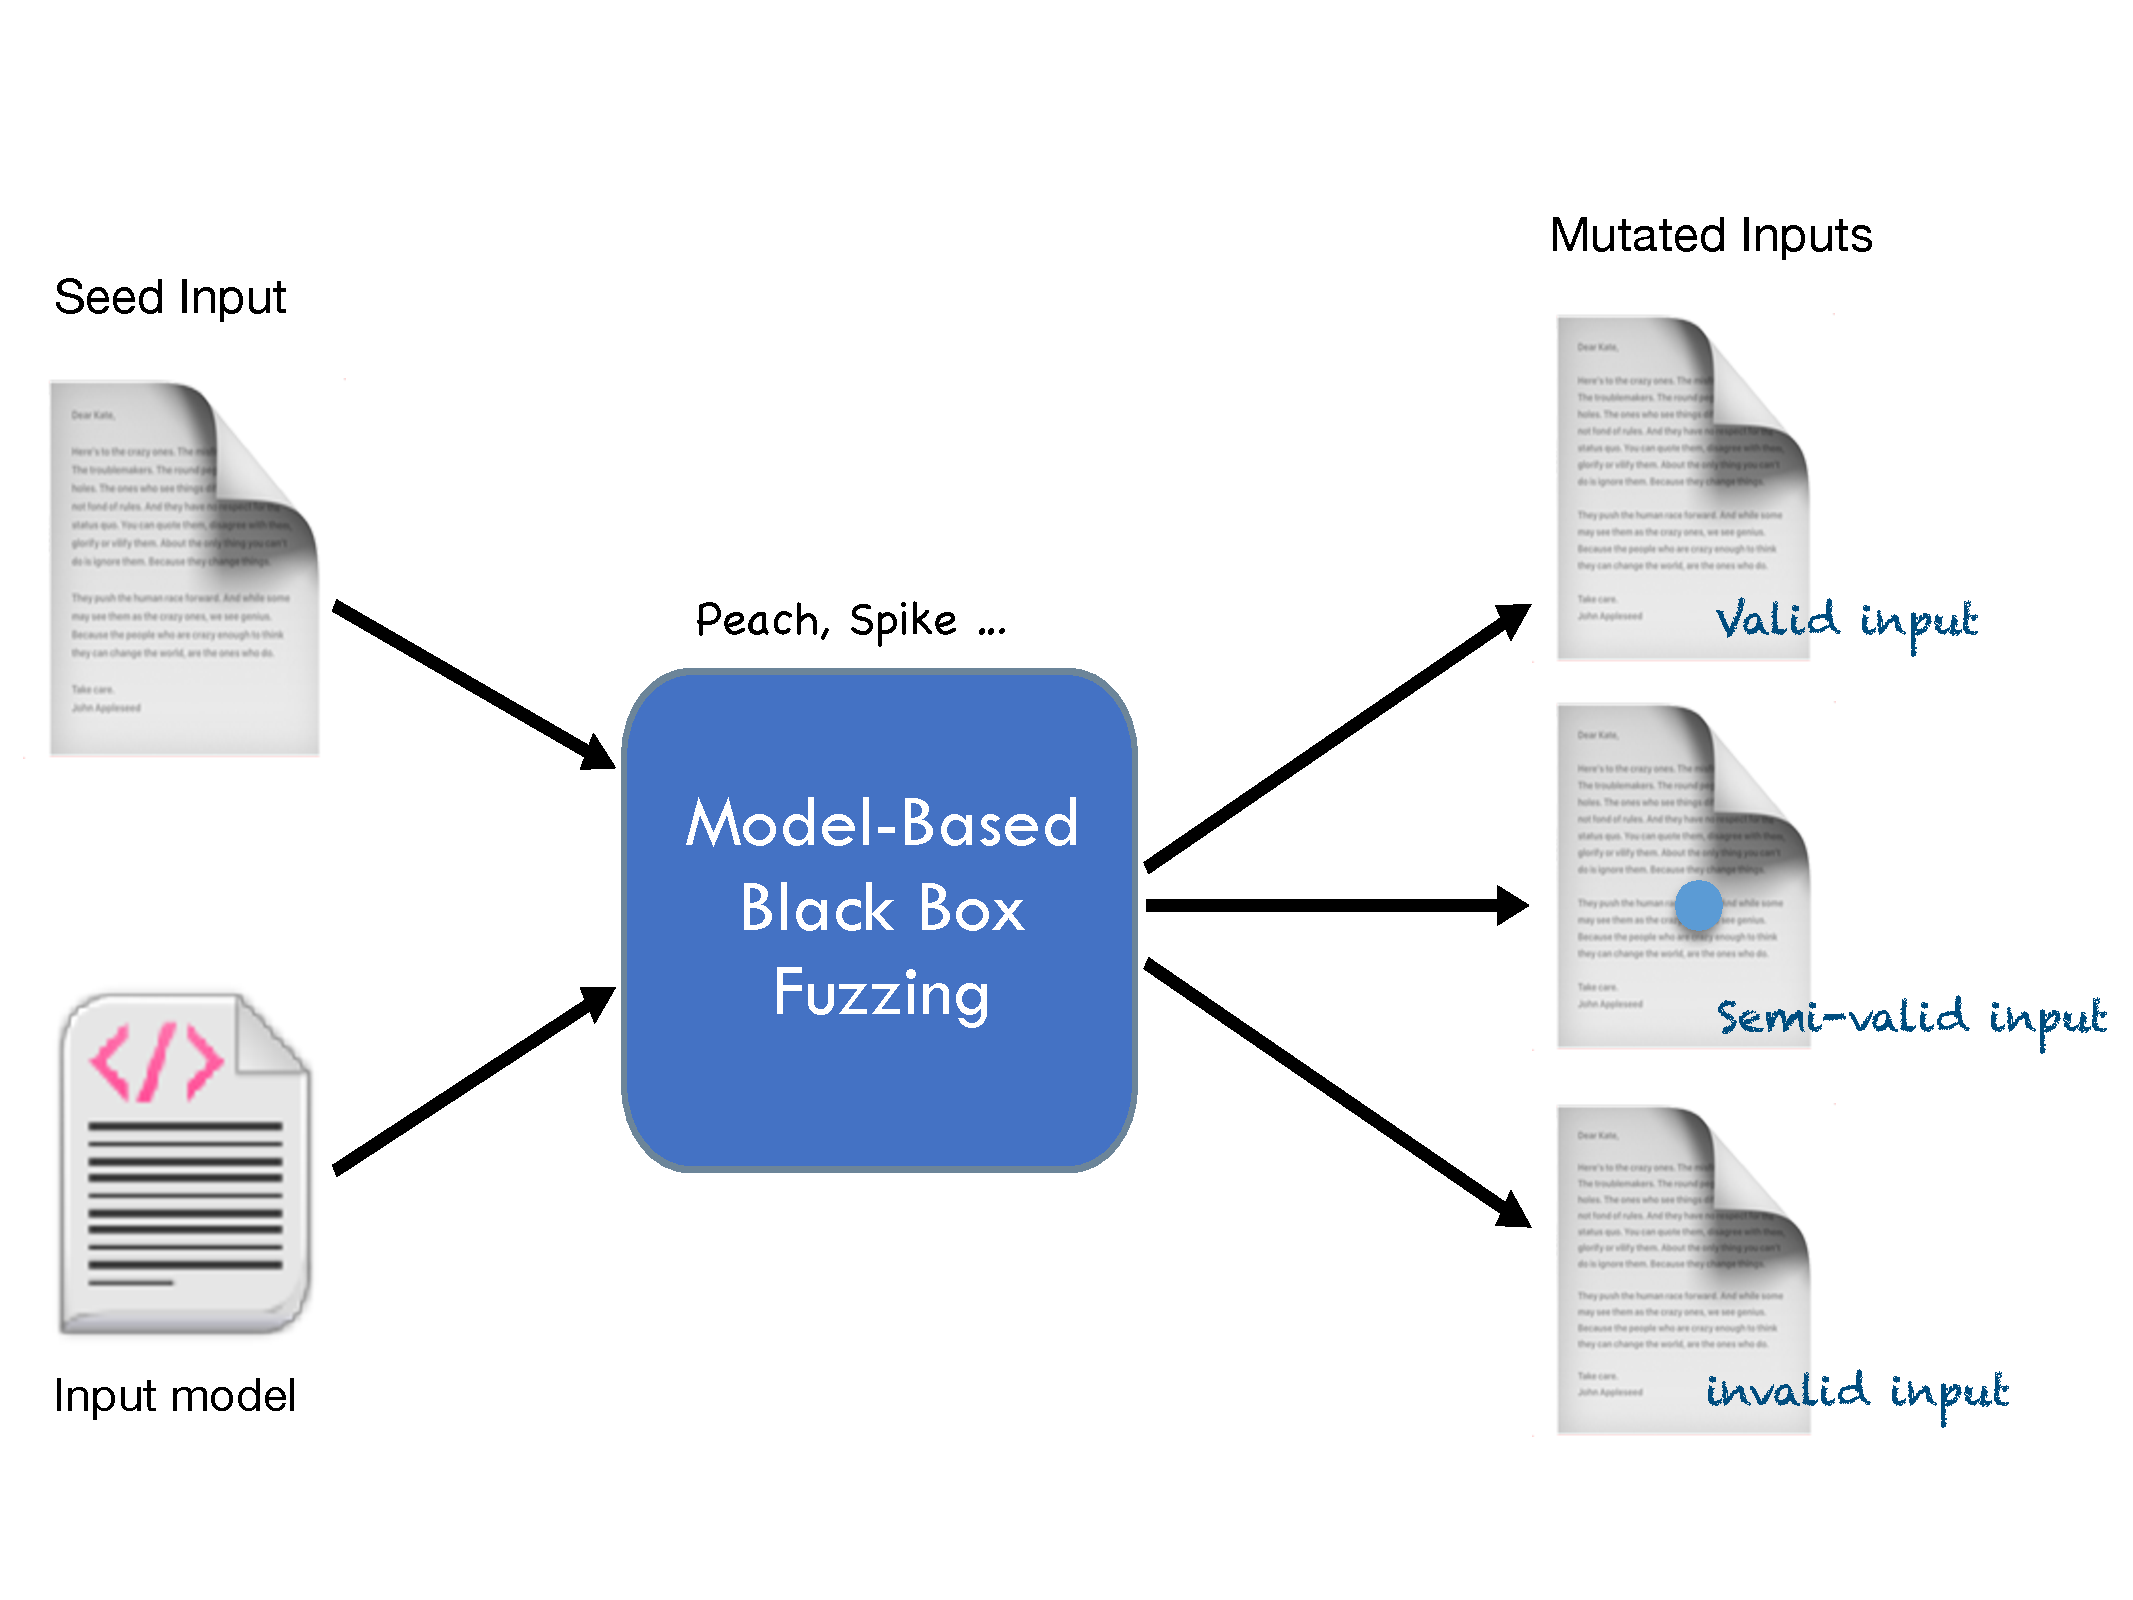
\includegraphics[width=8.0cm]{pic/blackbox.pdf}}
        \end{picture} 
    }

    \only<2>{
        \begin{itemize}  
        \item \structure {Black-box Fuzzing}
        \\ \textbf{Defination:} techniques that do not see the internals of the PUT,and can observe only the input/output behavior of the PUT,
           treating it as a black-box\cite{manes2019art}.
        \\ - No \alert{program analysis}, no \alert{feedback}
        \end{itemize} 
        \begin{picture}(320,250)
            \put(-25,110){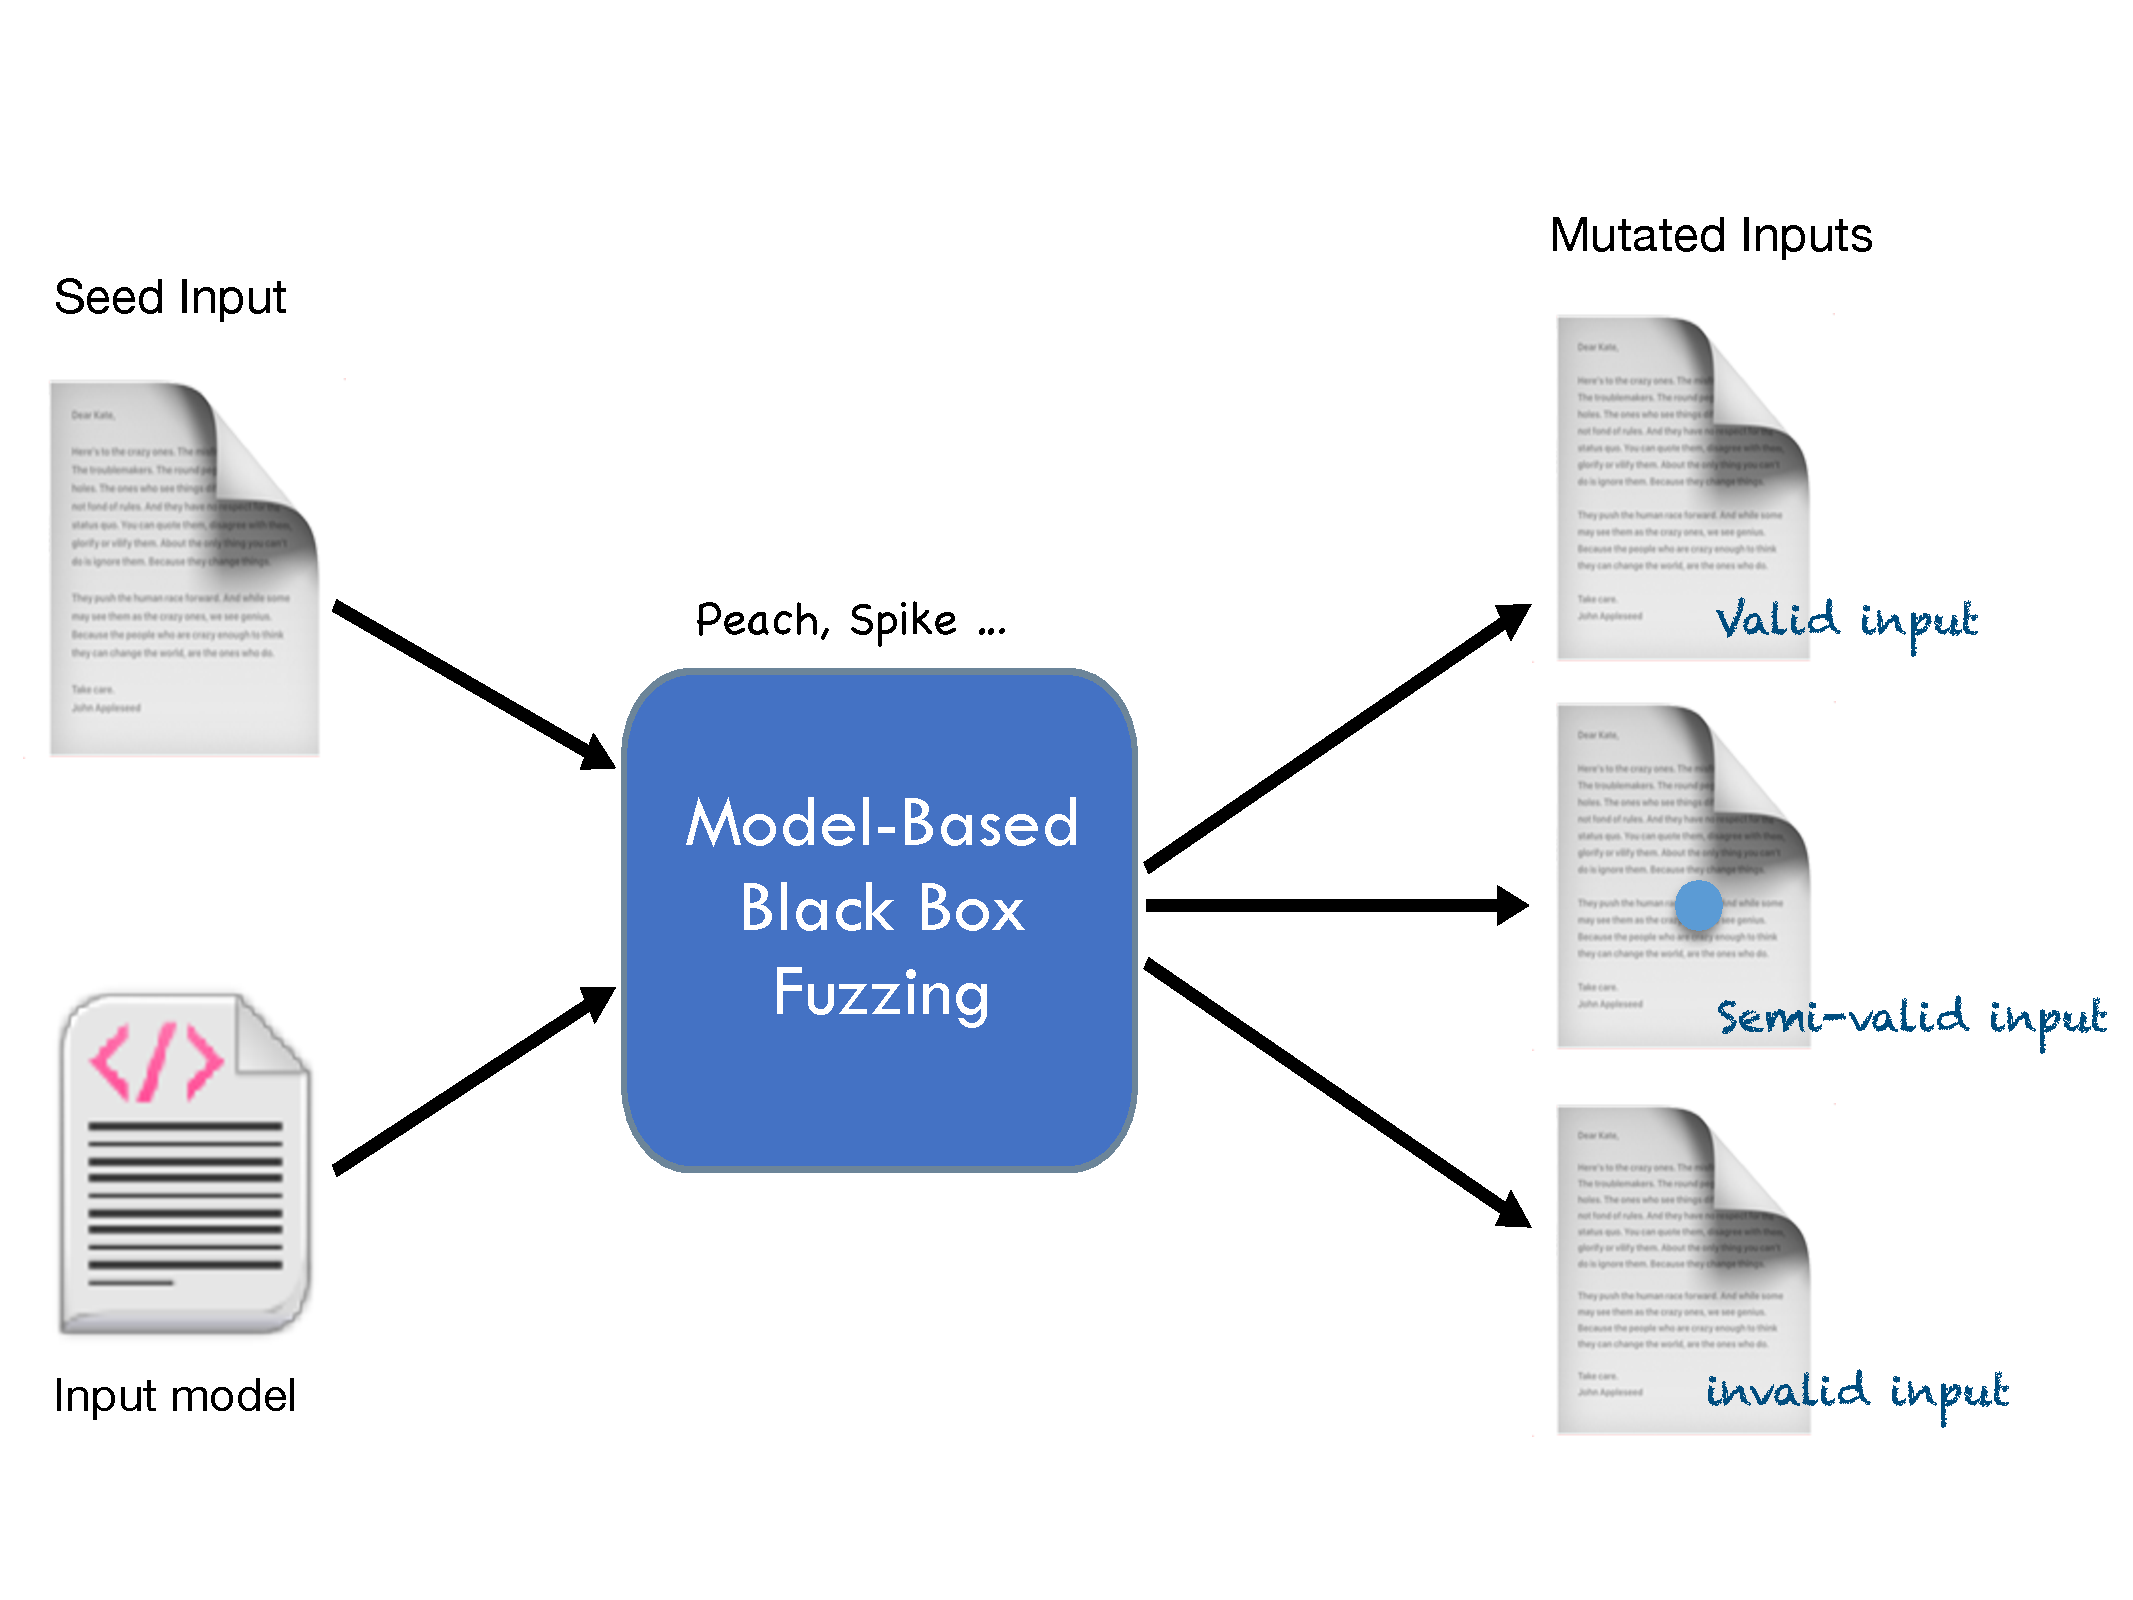
\includegraphics[width=8.0cm]{pic/blackbox.pdf}}
            \put(190,220){
                \begin{minipage}[t]{0.45\linewidth}
                {
                    \footnotesize{
                        \begin{itemize}  
                            \item  You have no view of the PUT,but have some view of the input/output domain
                            \item  Fuzzing process is not changed according to some feedback 
                            \item  Random mutated (not \alert {effective})
                        \end{itemize} 
                    }
                }
                \end{minipage}
                }
        \end{picture} 
    }
    \only<3>{
        \begin{itemize}  
        \item \structure {White-box Fuzzing}
          \\ \textbf{Defination:} techniques that generates test cases by analyzing the internals of the PUT and the information gathered 
          when executing the PUT\cite{manes2019art}.
          \\ - Requires heavy-weight \alert {program analysis} and constraint solving. 
        \end{itemize} 
        \begin{picture}(320,250)
            \put(-20,120){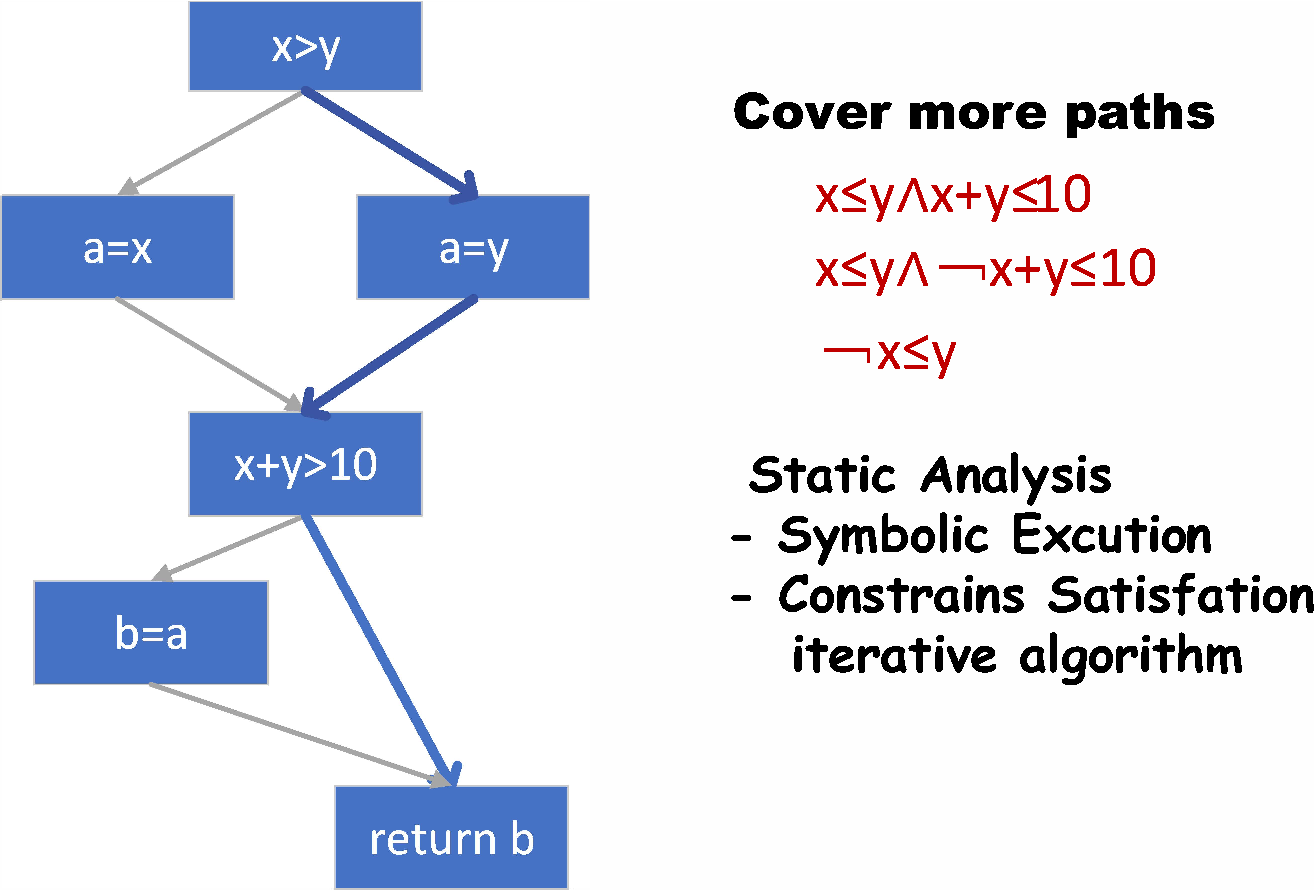
\includegraphics[width=6.0cm]{pic/cfg.pdf}}
            \put(160,120){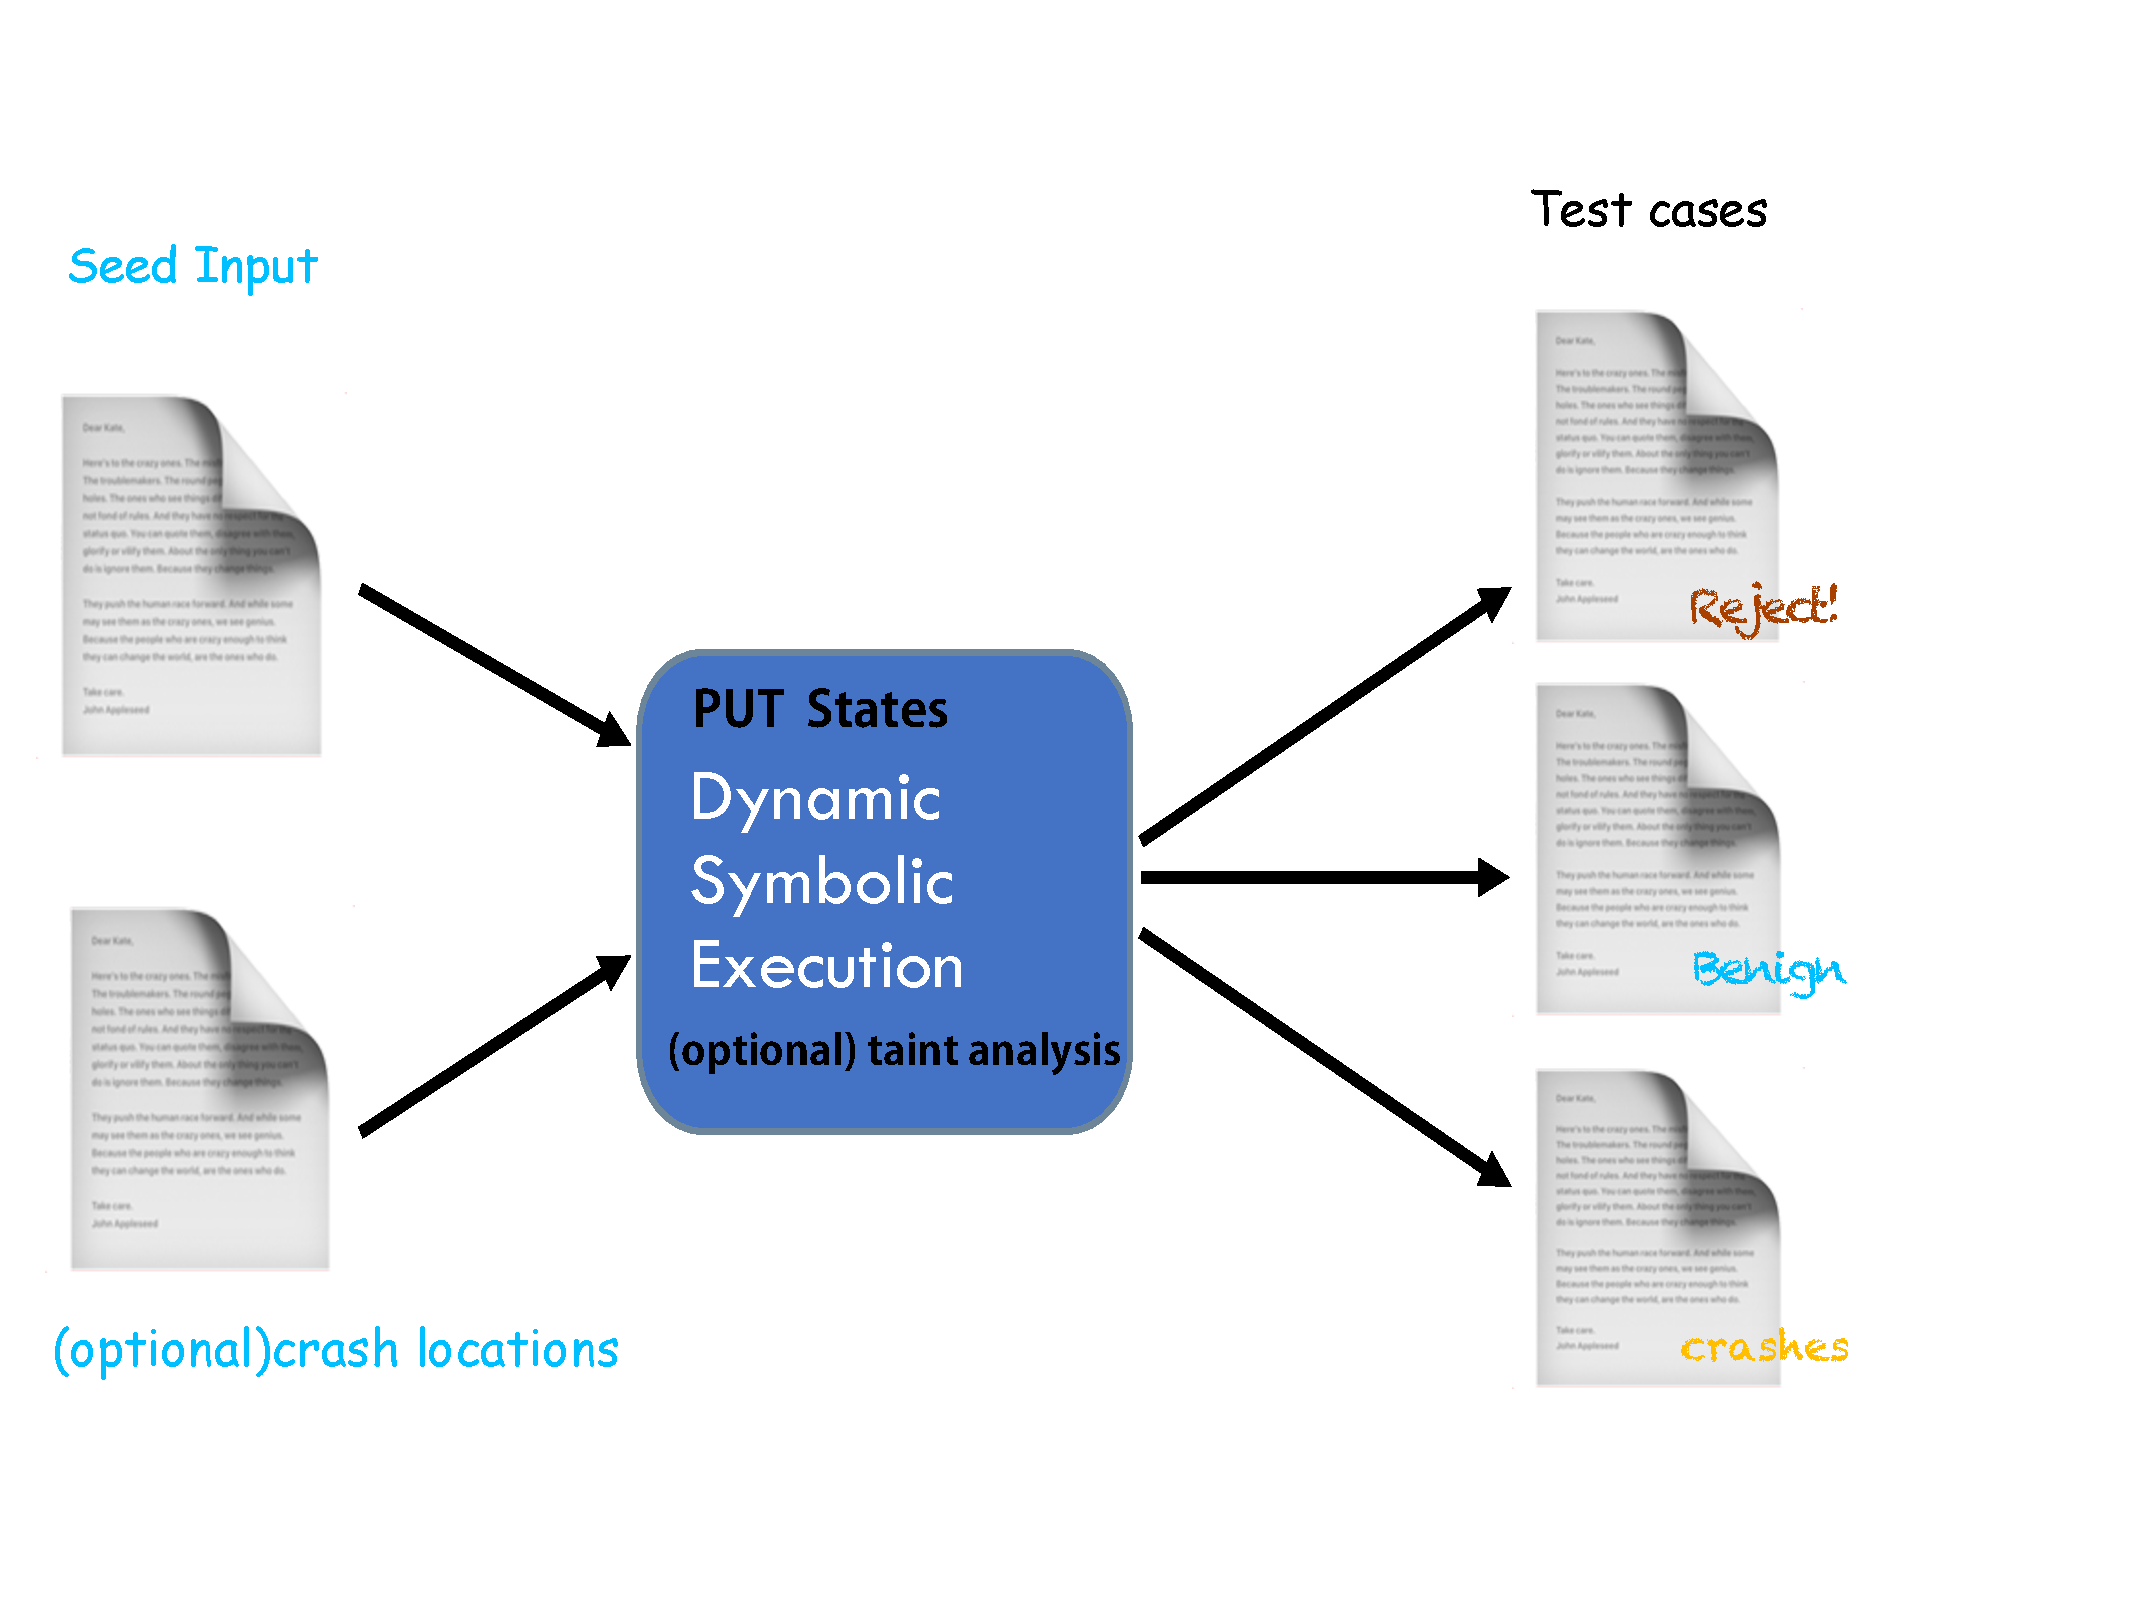
\includegraphics[width=6.0cm]{pic/whitebox.pdf}} 
        \end{picture} 
    }
    \only<4>{
        \begin{itemize}  
        \item \structure {White-box Fuzzing}
          \\ \textbf{Defination:} techniques that generates test cases by analyzing the internals of the PUT and the information gathered 
          when executing the PUT\cite{manes2019art}.
          \\ - Requires heavy-weight \alert {program analysis} and constraint solving. 
        \end{itemize}
        \begin{picture}(320,250) 
        \put(-15,110){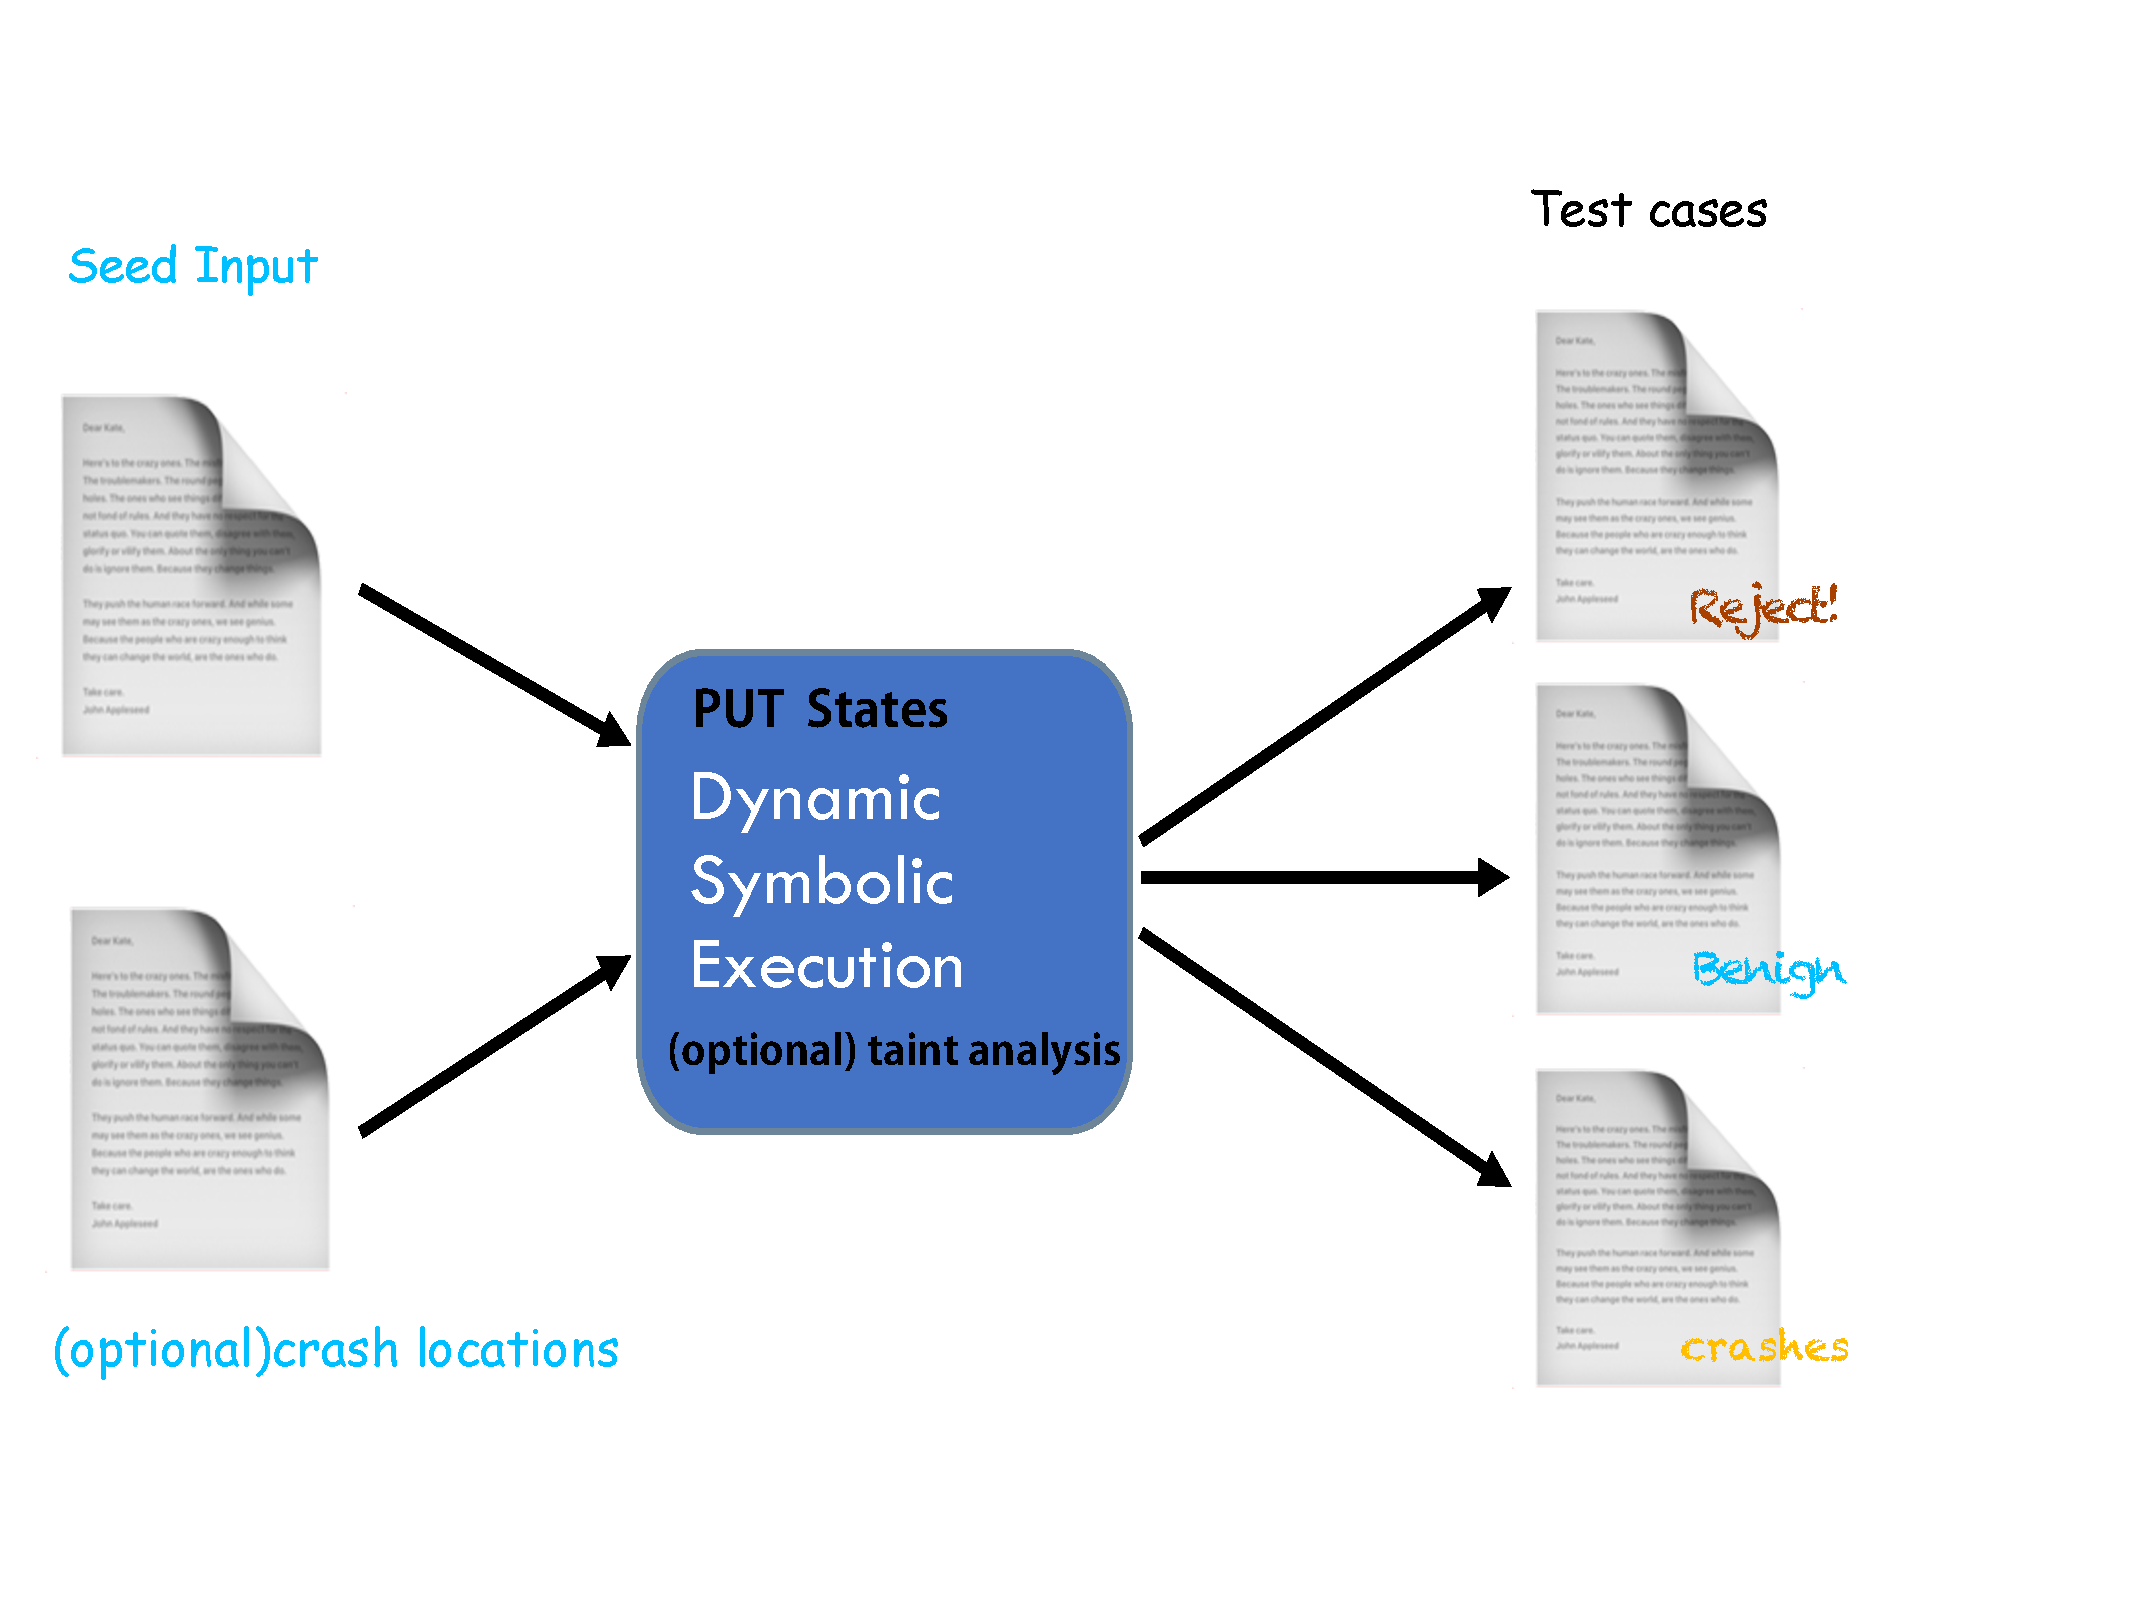
\includegraphics[width=8.0cm]{pic/whitebox.pdf}}
        \put(200,210){
            \begin{minipage}[t]{0.40\linewidth}
            {
                \footnotesize{
                    \begin{itemize}  
                        \item  You have the view of the PUT state(CFG,CG)
                        \item  Static analysis (effective but not \alert {efficient}!)
                    \end{itemize} 
                }
            }
            \end{minipage}
            }
    \end{picture} 
    }
    \only<5>{
        \begin{itemize}  
        \item \structure {Grey-box Fuzzing}
          \\ \textbf{Defination:} techniques that can obtain \textsl{some} information internal to the PUT and/or its executions to generates test cases\cite{manes2019art}.
          \\ - Uses only lightweight instrumentation to glean some program structure
          \\ - And coverage \alert{feedback} 
        \end{itemize} 
        \begin{figure}[htbp]
            \begin{center}
                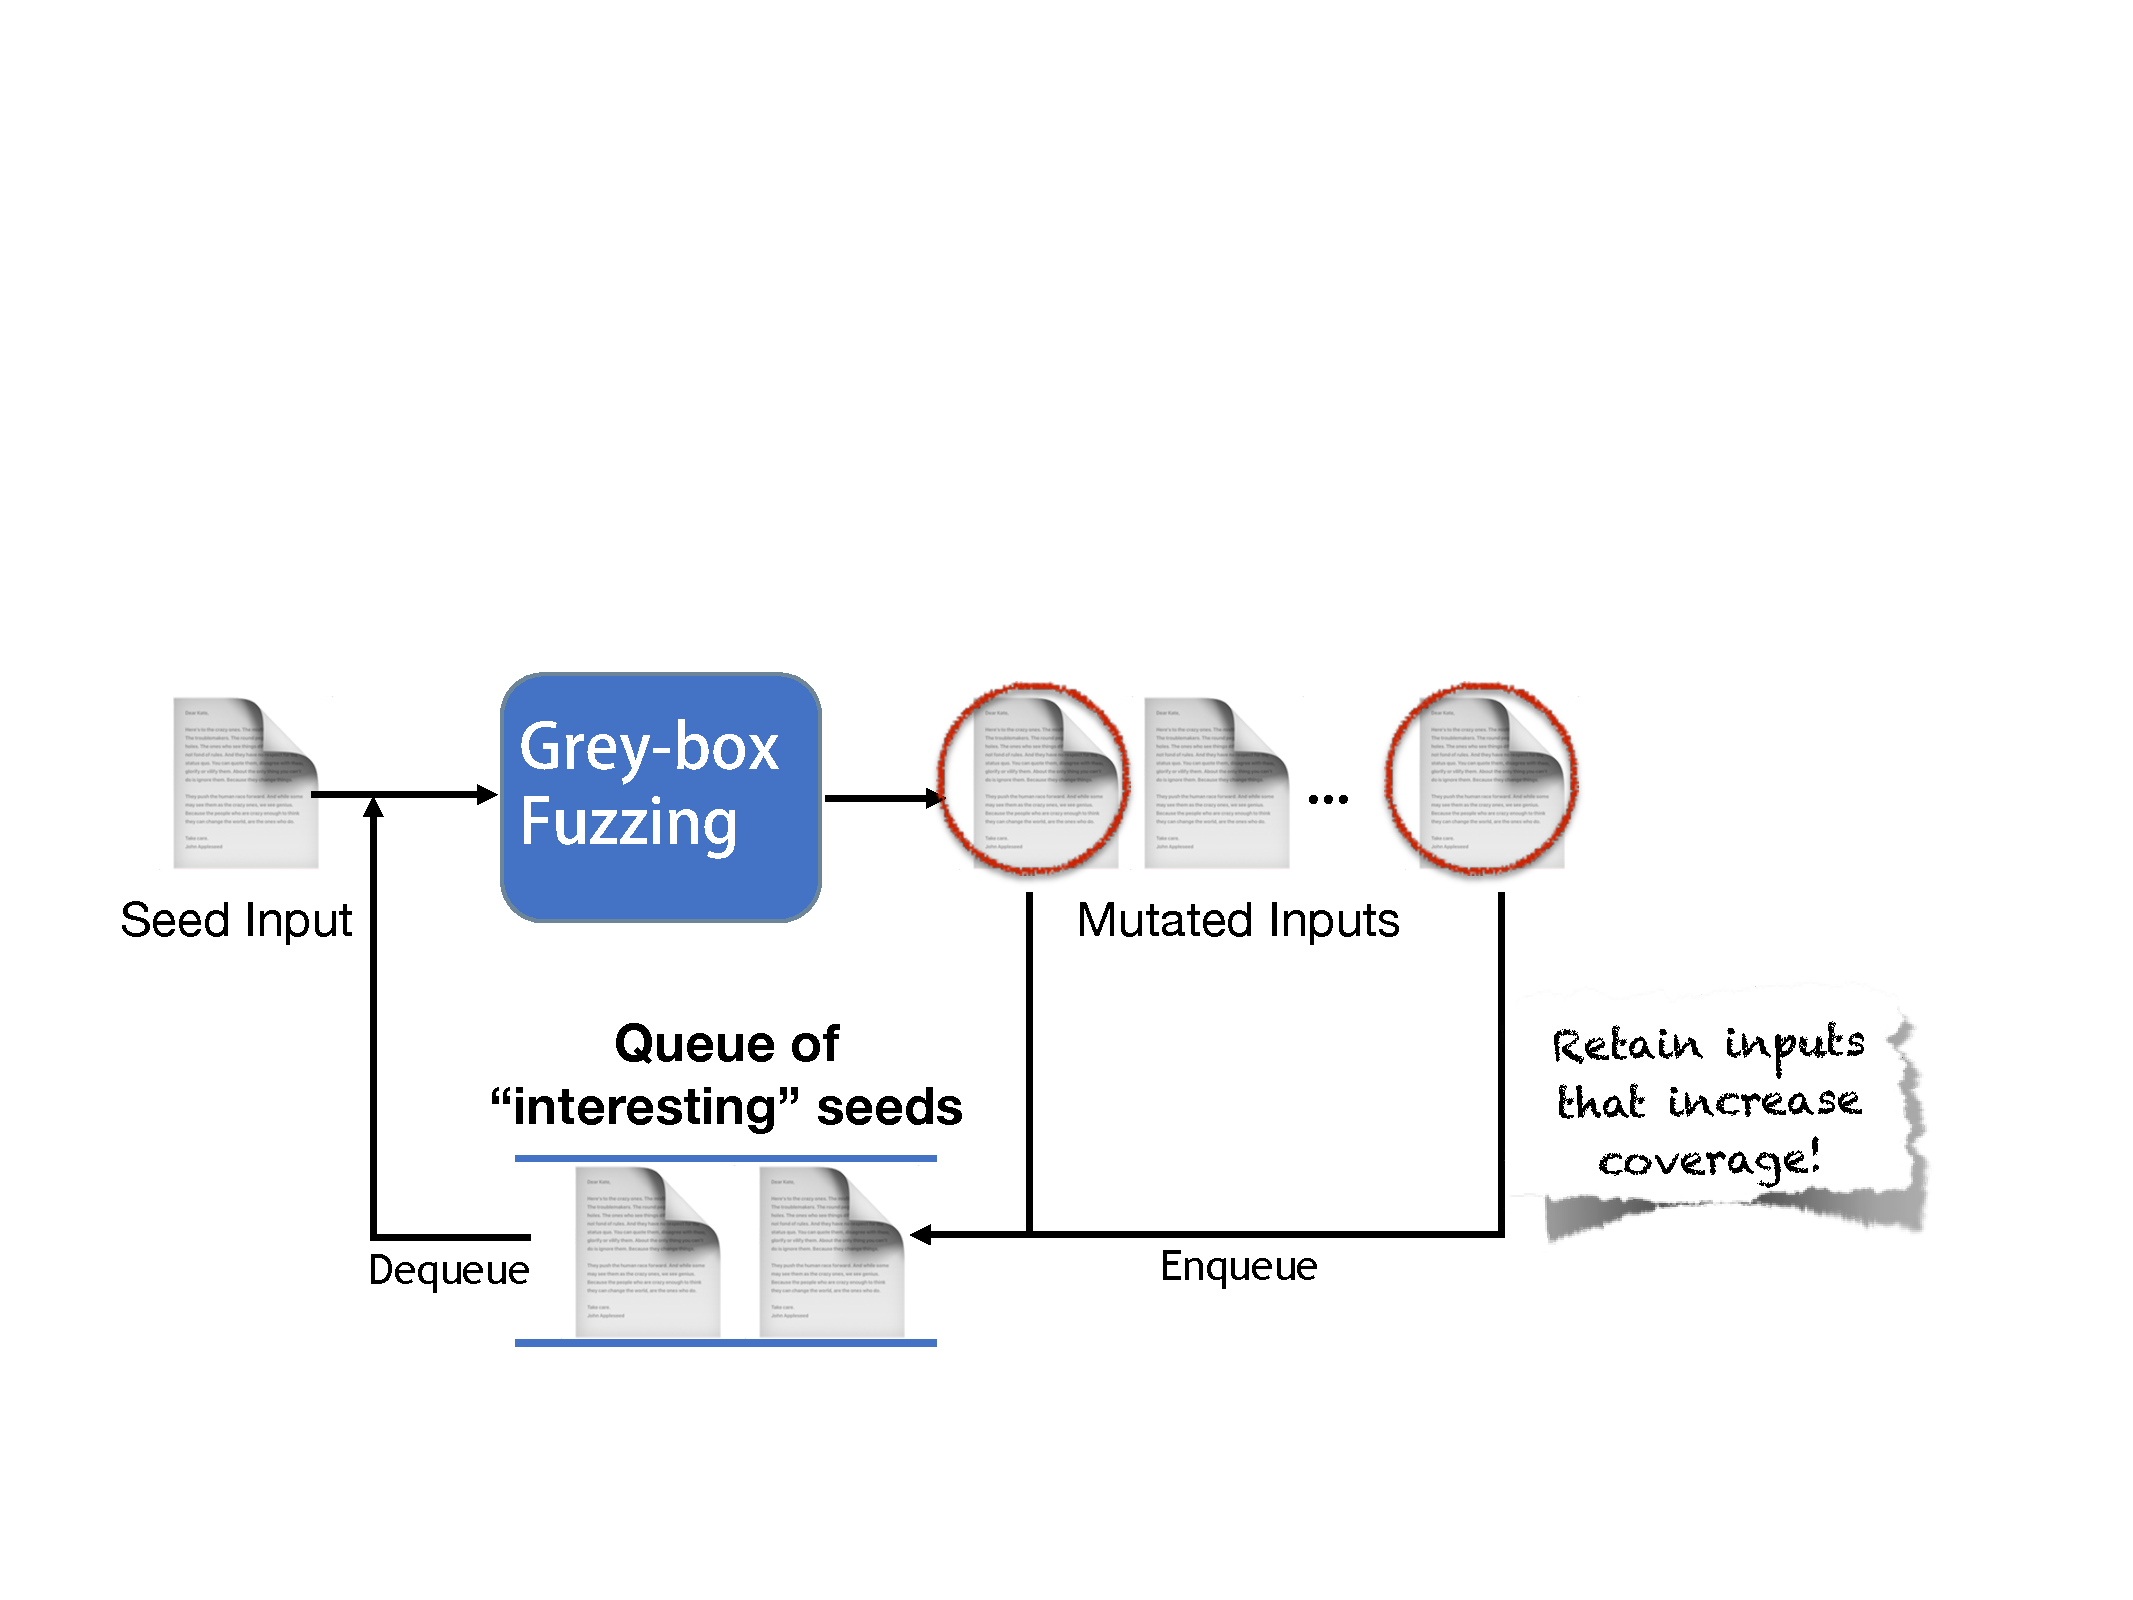
\includegraphics[width=10.0cm]{pic/greybox.pdf}
            \end{center}
        \end{figure} 
    }
\end{frame}
\begin{frame}{Why Directed Grey-box Fuzzing ?}
    
\end{frame}


\subsection{Research Status }
\begin{frame}{ Why Directed Grey-Box Fuzz?}
    \begin{itemize}[<+-| alert@+>] % 当然,除了alert,手动在里面插 \pause 也行
        \item 大家都会\LaTeX{},好多学校都有自己的Beamer主题
        \item 中文支持请选择 Xe\LaTeX{} 编译选项
    \end{itemize}
\end{frame}

% \section{研究内容}

% \subsection{美化主题}

% \begin{frame}{这一份主题与原始的THU Beamer Theme区别在于}
%     \begin{itemize}
%         \item 顶栏的小点变成一行而不是多行
%         \item 中文采用楷书
%         \item 修改了主题色为南邮校徽颜色
%         \item 参考文献格式按照毕设标准进行了修改
%         \item 更多该模板的功能可以参考 \url{https://www.latexstudio.net/archives/4051.html}
%         \item 下面列举出了一些Beamer的用法,部分节选自 \url{https://tuna.moe/event/2018/latex/}
%     \end{itemize}
% \end{frame}

% \subsection{如何更好地做Beamer}

% \begin{frame}{Why Beamer}
%     \begin{itemize}
%         \item \LaTeX 广泛用于学术界,期刊会议论文模板
%     \end{itemize}
%     \begin{table}[h]
%         \centering
%         \begin{tabular}{c|c}
%             Microsoft\textsuperscript{\textregistered}  Word & \LaTeX \\
%             \hline
%             文字处理工具 & 专业排版软件 \\
%             容易上手,简单直观 & 容易上手 \\
%             所见即所得 & 所见即所想,所想即所得 \\
%             高级功能不易掌握 & 进阶难,但一般用不到 \\
%             处理长文档需要丰富经验 & 和短文档处理基本无异 \\
%             花费大量时间调格式 & 无需担心格式,专心作者内容 \\
%             公式排版差强人意 & 尤其擅长公式排版 \\
%             二进制格式,兼容性差 & 文本文件,易读、稳定 \\
%             付费商业许可 & 自由免费使用 \\
%         \end{tabular}
%     \end{table}
% \end{frame}

% \begin{frame}{排版举例}
%     \begin{exampleblock}{无编号公式} % 加 * 
%         \begin{equation*}
%             J(\theta) = \mathbb{E}_{\pi_\theta}[G_t] = \sum_{s\in\mathcal{S}} d^\pi (s)V^\pi(s)=\sum_{s\in\mathcal{S}} d^\pi(s)\sum_{a\in\mathcal{A}}\pi_\theta(a|s)Q^\pi(s,a)
%         \end{equation*}
%     \end{exampleblock}
%     \begin{exampleblock}{多行多列公式\footnote{如果公式中有文字出现,请用 $\backslash$mathrm\{\} 或者 $\backslash$text\{\} 包含,不然就会变成 $clip$,在公式里看起来比 $\mathrm{clip}$ 丑非常多。}}
%         % 使用 & 分隔
%         \begin{align}
%             Q_\mathrm{target}&=r+\gamma Q^\pi(s^\prime, \pi_\theta(s^\prime)+\epsilon)\\
%             \epsilon&\sim\mathrm{clip}(\mathcal{N}(0, \sigma), -c, c)\nonumber
%         \end{align}
%     \end{exampleblock}
% \end{frame}

% \begin{frame}
%     \begin{exampleblock}{编号多行公式}
%         % Taken from Mathmode.tex
%         \begin{multline}
%             A=\lim_{n\rightarrow\infty}\Delta x\left(a^{2}+\left(a^{2}+2a\Delta x+\left(\Delta x\right)^{2}\right)\right.\label{eq:reset}\\
%             +\left(a^{2}+2\cdot2a\Delta x+2^{2}\left(\Delta x\right)^{2}\right)\\
%             +\left(a^{2}+2\cdot3a\Delta x+3^{2}\left(\Delta x\right)^{2}\right)\\
%             +\ldots\\
%             \left.+\left(a^{2}+2\cdot(n-1)a\Delta x+(n-1)^{2}\left(\Delta x\right)^{2}\right)\right)\\
%             =\frac{1}{3}\left(b^{3}-a^{3}\right)
%         \end{multline}
%     \end{exampleblock}
% \end{frame}


% \begin{frame}[fragile]{\LaTeX{} 常用命令}
%     \begin{exampleblock}{命令}
%         \centering
%         \footnotesize
%         \begin{tabular}{llll}
%             \cmd{chapter} & \cmd{section} & \cmd{subsection} & \cmd{paragraph} \\
%             章 & 节 & 小节 & 带题头段落 \\\hline
%             \cmd{centering} & \cmd{emph} & \cmd{verb} & \cmd{url} \\
%             居中对齐 & 强调 & 原样输出 & 超链接 \\\hline
%             \cmd{footnote} & \cmd{item} & \cmd{caption} & \cmd{includegraphics} \\
%             脚注 & 列表条目 & 标题 & 插入图片 \\\hline
%             \cmd{label} & \cmd{cite} & \cmd{ref} \\
%             标号 & 引用参考文献 & 引用图表公式等\\\hline
%         \end{tabular}
%     \end{exampleblock}
%     \begin{exampleblock}{环境}
%         \centering
%         \footnotesize
%         \begin{tabular}{lll}
%             \env{table} & \env{figure} & \env{equation}\\
%             表格 & 图片 & 公式 \\\hline
%             \env{itemize} & \env{enumerate} & \env{description}\\
%             无编号列表 & 编号列表 & 描述 \\\hline
%         \end{tabular}
%     \end{exampleblock}
% \end{frame}

% \begin{frame}[fragile]{\LaTeX{} 环境命令举例}
%     \begin{minipage}{0.5\linewidth}
% \begin{lstlisting}[language=TeX]
% \begin{itemize}
%   \item A \item B
%   \item C
%   \begin{itemize}
%     \item C-1
%   \end{itemize}
% \end{itemize}
% \end{lstlisting}
%     \end{minipage}\hspace{1cm}
%     \begin{minipage}{0.3\linewidth}
%         \begin{itemize}
%             \item A
%             \item B
%             \item C
%             \begin{itemize}
%                 \item C-1
%             \end{itemize}
%         \end{itemize}
%     \end{minipage}
%     \medskip
%     \pause
%     \begin{minipage}{0.5\linewidth}
% \begin{lstlisting}[language=TeX]
% \begin{enumerate}
%   \item 巨佬 \item 大佬
%   \item 萌新
%   \begin{itemize}
%     \item[n+e] 瑟瑟发抖
%   \end{itemize}
% \end{enumerate}
% \end{lstlisting}
%     \end{minipage}\hspace{1cm}
%     \begin{minipage}{0.3\linewidth}
%         \begin{enumerate}
%             \item 巨佬
%             \item 大佬
%             \item 萌新
%             \begin{itemize}
%                 \item[n+e] 瑟瑟发抖
%             \end{itemize}
%         \end{enumerate}
%     \end{minipage}
% \end{frame}

% \begin{frame}[fragile]{\LaTeX{} 数学公式}
%     \begin{columns}
%         \begin{column}{.55\textwidth}
% \begin{lstlisting}[language=TeX]
% $V = \frac{4}{3}\pi r^3$

% \[
%   V = \frac{4}{3}\pi r^3
% \]

% \begin{equation}
%   \label{eq:vsphere}
%   V = \frac{4}{3}\pi r^3
% \end{equation}
% \end{lstlisting}
%         \end{column}
%         \begin{column}{.4\textwidth}
%             $V = \frac{4}{3}\pi r^3$
%             \[
%                 V = \frac{4}{3}\pi r^3
%             \]
%             \begin{equation}
%                 \label{eq:vsphere}
%                 V = \frac{4}{3}\pi r^3
%             \end{equation}
%         \end{column}
%     \end{columns}
%     \begin{itemize}
%         \item 更多内容请看 \href{https://zh.wikipedia.org/wiki/Help:数学公式}{\color{purple}{这里}}
%     \end{itemize}
% \end{frame}

% \begin{frame}[fragile]
%     \begin{columns}
%         \column{.6\textwidth}
% \begin{lstlisting}[language=TeX]
%     \begin{table}[htbp]
%       \caption{编号与含义}
%       \label{tab:number}
%       \centering
%       \begin{tabular}{cl}
%         \toprule
%         编号 & 含义 \\
%         \midrule
%         1 & 4.0 \\
%         2 & 3.7 \\
%         \bottomrule
%       \end{tabular}
%     \end{table}
%     公式~(\ref{eq:vsphere}) 的
%     编号与含义请参见
%     表~\ref{tab:number}。
% \end{lstlisting}
%         \column{.4\textwidth}
%         \begin{table}[htpb]
%             \centering
%             \caption{编号与含义}
%             \label{tab:number}
%             \begin{tabular}{cl}\toprule
%                 编号 & 含义 \\\midrule
%                 1 & 4.0\\
%                 2 & 3.7\\\bottomrule
%             \end{tabular}
%         \end{table}
%         \normalsize 公式~(\ref{eq:vsphere})的编号与含义请参见表~\ref{tab:number}。
%     \end{columns}
% \end{frame}

% \begin{frame}{作图}
%     \begin{itemize}
%         \item 矢量图 eps, ps, pdf
%         \begin{itemize}
%             \item METAPOST, pstricks, pgf $\ldots$
%             \item Xfig, Dia, Visio, Inkscape $\ldots$
%             \item Matlab / Excel 等保存为 pdf
%         \end{itemize}
%         \item 标量图 png, jpg, tiff $\ldots$
%         \begin{itemize}
%             \item 提高清晰度,避免发虚
%             \item 应尽量避免使用
%         \end{itemize}
%     \end{itemize}
%     \begin{figure}[htpb]
%         \centering
%         
\includegraphics[width=0.2\linewidth]{pic/NJUPT_Logo.pdf
%         }
%         \caption{这个校徽就是矢量图,虽然看起来不像,但确实是矢量图格式}
%     \end{figure}
% \end{frame}

% \section{计划进度}
% \begin{frame}
%     \begin{itemize}
%         \item 一月:完成文献调研
%         \item 二月:研究THU Beamer Theme的实现
%         \item 三、四月:修改NJUPT Beamer主题
%         \item 五月:论文撰写
%     \end{itemize}
% \end{frame}

 \section{参考文献}

 \begin{frame}[allowframebreaks]
     \bibliography{ref}
     \bibliographystyle{gbt}
 \end{frame}

 \begin{frame}
     \begin{center}
         {\Huge Thanks!}
     \end{center}
 \end{frame}

 \end{document}